\subsection{Definition of the Integral}
\subsubsection{Antidifferentiation}
The antiderivative is the reverse of the derivative and is found by integration. When we integrate, we must include an arbitrary constant $C$, in order to include every possible antiderivative in our solution. This is because the derivative of a constant is always 0.
$$\int f(x)dx=F(x)+C$$
Many of the elementary functions have antiderivatives that are relatively simple to compute:
\begin{align*}
    &\int x^ndx=\frac{x^{n+1}}{n+1}+C\\
    &\int \frac{dx}{x}=\ln|x|+C\\
    &\int \sin{x} dx=-\cos x+C\\
    &\int \cos{x} dx=\sin x+C\\
    &\int e^xdx=e^x+C
\end{align*}
Ex: $\int xdx=\frac{1}{2}x^2+C$\\
\subsubsection{Numeric Integration}
Riemann Sums:
The integral of a function is analogous to the area under the curve. This can be shown using Riemann Sums.\\
We can express the area under a curve by breaking up the area into a series of rectangles.\\
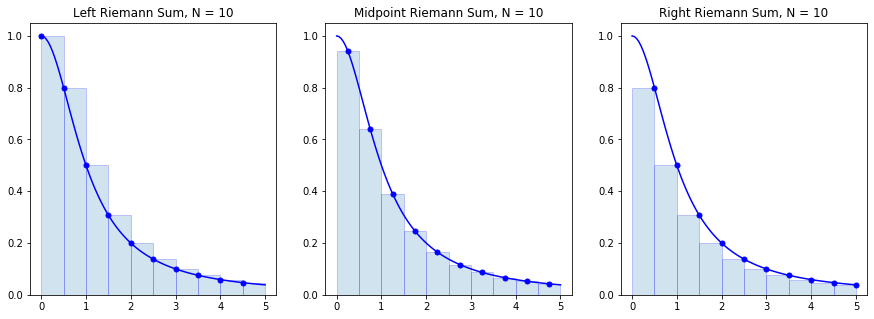
\includegraphics[scale=0.57]{Images/IntegralCalcPictures/RiemannSums.png}\\
For the area under the curve $y=x$ between 0 and 1, if we break it up into 4 sections, the width of each rectangle will be $\frac{1}{4}$. The height of the rectangles will depend on whether you take left, right, or mid endpoints. Taking left endpoints, the heights will be $0,\,\frac{1}{4},\,\frac{1}{2},\,\frac{3}{4}$. So the total area is the sum of the 4 rectangles, $A=0+\frac{1}{16}+\frac{1}{8}+\frac{3}{16}=\frac{3}{8}$ which is close to the actual value of $\frac{1}{2}$.\\
In general, the area under a curve can be expressed as
$$A\approx\sum_{i=1}^nf(x_i^*)\Delta x$$
$\Delta x$ is the width of the rectangles. where 
\begin{align*}
    &\Delta x =\frac{b-a}{n}
\end{align*}
and $x_i^*$ refers to the position of the rectangle and the end points.
\begin{align*}
    \text{Right: }&x_i^*=a+i\Delta x\\
    \text{Left: }&x_i^*=a+(i-1)\Delta x\\
    \text{Mid: }&x_i^*=a+\brround{i-\frac{1}{2}}\Delta x
\end{align*}
The more rectangles we use, the better the approximation. As we take the limit as $n\to\infty$, we will get an exact value for the area.
Ex: Area of $y=x$ between 0 and 1.
\begin{align*}
    &A=\lim_{n\to\infty}\sum_{i=1}^nf(x_i^*)\Delta x\\
    &\Delta x=\frac{1-0}{n}\\
    &x_i^*=i\Delta x=\frac{i}{n}\\
    &A=\lim_{n\to\infty}\sum_{i=1}^n\frac{i}{n^2}=\lim_{n\to\infty}\frac{1}{n^2}\sum_{i=1}^ni\\
\end{align*}
We have the following formulas in order to express sums
\begin{align*}
    \sum_{i=1}^n1&=n\\
    \sum_{i=1}^ni&=\frac{n(n+1)}{2}\\
    \sum_{i=1}^ni^2&=\frac{n(n+1)(2n+1)}{6}\\
    \sum_{i=1}^ni^3&=\frac{n^2(n+1)^2}{4}
\end{align*}
So we can express the area in our example as
\begin{align*}
    A&=\lim_{n\to\infty}\frac{1}{n^2}\sum_{i=1}^ni=\lim_{n\to\infty}\frac{n(n+1)}{2n^2}=\lim_{n\to\infty}\frac{n^2}{2n^2}+\frac{n}{2n^2}=\frac{1}{2}+\lim_{n\to\infty}\frac{1}{2n}\\
    &=\frac{1}{2}
\end{align*}
which fits with what we expect\\
An important thing to note is that the area under a curve can come out negative if the function is below the x-axis.\\
Ex2: Find the area under the curve $f(t)=t^2$ between 0 and some number $x$.
\begin{align*}
    &\Delta t=\frac{x}{n}\\
    &x_i^*=\frac{ix}{n}\\
    &A=\lim_{n\to\infty}\sum_{i=1}^n\frac{i^2x^3}{n^3}=\lim_{n\to\infty}\frac{x^3}{n^3}\sum_{i=1}^ni^2\\
    &A=\lim_{n\to\infty}\frac{x^3}{n^3}\cdot\frac{n(n+1)(2n+1)}{6}\\
    &A=\lim_{n\to\infty}\frac{x^3}{3}+\frac{1}{2n}+\frac{1}{6n^2}=\frac{x^3}{3}
\end{align*}
Notice this is the same as the antiderivative $\int x^2dx=\frac{x^3}{3}$ so we can see that the integral is analogous to the area under the curve.\\

Another method of numeric integration is the trapezoidal method where instead of using rectangles, we use trapezoids to form the area.
$$\Delta A=\Delta x\brround{\frac{y_0+y_1}{2}}$$
This happens to be identical to taking midpoints using Riemann sums.\\
A better method of numerical integration is Simpson's Rule:\\
This involves using the area under a parabola as a basis for approximation.
$$\Delta A=2\Delta x\brround{\frac{y_0+4y_1+y_2}{6}}$$
Where $2\Delta x$ is the base and $\dfrac{y_0+4y_1+y_2}{6}$ is the average height of the parabola. This works out to be
$$A=\frac{\Delta x}{3}(y_0+4y_1+2y_2+4y_3+\cdots+2y_{n-2}+4y_{n-1}+y_n)$$
Note that for Simpson's rule, we require that $n$ be an even number.\\
Ex: Estimate $\int_0^\pi\sin xdx$ using $n=4$\\
\begin{tabular}{c|c|c}
    $i$ & $x_i$ & $f(x_i)$\\
    \hline
    0 & 0 & 0\\
    1 & $\frac{\pi}{4}$ & $\frac{\sqrt{2}}{2}$\\
    2 & $\frac{\pi}{2}$ & 1\\
    3 & $\frac{3\pi}{4}$ & $\frac{\sqrt{2}}{2}$\\
    4 & $\pi$ & 0
\end{tabular}\\
\begin{align*}
    A=&\frac{\Delta x}{3}(y_0+4y_1+2y_2+4y_3+y_4)\\
    &=\frac{\pi}{12}(0+2\sqrt{2}+2+2\sqrt{2}+0)=\frac{\pi}{6}(1+2\sqrt{2})
\end{align*}
\subsubsection{The Definite Integral}
We can define the definite integral as the infinite sum of the area and can be written as
$$\int_a^bf(x)dx=\lim_{n\to\infty}\sum_{i=1}^nf(x_i^*)\Delta x$$
We can convert infinite sums to integral form by identifying the bounds and the function. Some things to look for are:
\begin{itemize}
    \item look for $\frac{i^*}{n}$ combos to spot $x_i$
    \item look for an additional $\frac{1}{n}$ term on the outside of the function to spot $\Delta x$
\end{itemize}
\begin{align*}
    \text{Ex: }&\lim_{n\to\infty}\sum_{i=1}^n\frac{\sqrt{i^2+9n^2}}{i^2}\\
    &I=\lim_{n\to\infty}\sum_{i=1}^n\sqrt{\frac{1}{i^2}+\frac{9n^2}{i^4}}\\
    &I=\lim_{n\to\infty}\sum_{i=1}^n\frac{1}{n}\sqrt{\frac{n^2}{i^2}+\frac{9n^4}{i^4}}\\
    &\text{assume }\Delta x=\frac{1}{n},\,x_i^*=\frac{i}{n}\\
    &I=\int_0^1\sqrt{\frac{1}{x^2}+\frac{9}{x^4}}dx=\int_0^1\frac{\sqrt{x^2+9}}{x^2}dx
\end{align*}
Note for these problems there are multiple different solutions. i.e. choosing left-hand end points vs. right-hand end points will give different answers.\\

Integral Properties:\\
Integrals have all the usual addition/subtraction properties as well as some other useful identities:
\begin{align*}
    &\int_a^af(x)dx=0\\
    &\int_a^bf(x)dx=-\int_b^af(x)dx\\
    &\int_a^bf(x)dx=\int_a^cf(x)dx+\int_c^bf(x)dx\\
    &\text{if $f(x)$ is even, }\int_{-a}^af(x)dx=2\int_0^af(x)dx\\
    &\text{if $f(x)$ is odd, }\int_{-a}^af(x)dx=0
\end{align*}

Fundamental Theorem of Calculus 1:
We have seen how the area under a curve is related to the antiderivative of the curve. This is expressed in the FTC1
$$\int_a^b f(x)dx=F(b)-F(a)=\left.F(x)\right|^b_a=\brsquare{F(x)}^b_a$$
\begin{align*}
    \text{Ex: }\int_0^12xdx=\left.x^2\right|_0^1=1^2-0^2=1
\end{align*}
In some situations, you may be required to break the function into separate integrals in order to evaluate them.
\begin{align*}
    \text{Ex2: }&\int_{-2}^1|2x-1|dx\\
    &I=\int_{-2}^{\frac{1}{2}}(1-2x)dx+\int_{\frac{1}{2}}^1(2x-1)dx\\
    &I=\brsquare{x-x^2}_{-2}^{1/2}+\brsquare{x^2-x}_{1/2}^1=6.5
\end{align*}

\subsubsection{Transcendental Functions}
We have seen transcendental numbers such as $\pi$ or $\sqrt{2}$. They are numbers that are described in terms of themselves and cannot be expressed in terms of what we already know. This same thing can be done with functions. $\sin x$ and $\ln x$ are examples of transcendental functions. With the Second Fundamental Theorem of Calculus, we are able to create more transcendental functions.\\
The 2nd Fundamental Theorem (FTC2) is known as
$$f(x)=\frac{d}{dx}\int_a^xf(t)dt$$
We can express the derivatives of these functions using the FTC1 and chain rule:\\
\begin{align*}
    F(x)=\displaystyle{\int^{u(x)}_{v(x)}f(x)dx}=F(u)-F(v)\\
    F'(x)=f(u)u'-f(v)v'
\end{align*}
\begin{align*}
    \text{Ex: }&\frac{d}{dx}\int_x^{x^2}\cos t dt=2x\cos x^2-\cos x
\end{align*}
While we always know the derivative of an integral, not all integrals themselves are solvable. The ones that aren't solvable are where we can come up with transcendental functions and we can use the information from its derivative to figure out what it may look like
\begin{align*}
    \text{Ex: }&f(x)=\int_1^x\frac{dt}{t}\\
    &f(1)=\int_1^1\frac{dt}{t}=0\\
    &f'(x)=\frac{1}{x}\Ra\text{increasing for }x>0\\
    &f''(x)=-\frac{1}{x^2}\Ra\text{concave up for all }x
\end{align*}
This function, you may recognize, is the definition of $\ln x$
\begin{align*}
    \text{Ex2: }&f(x)=\int_0^xe^{-t^2}dt\\
    &f(0)=0\\
    &f'(x)=e^{-x^2}\Ra\text{always increasing}\\
    &f'(0)=1\\
    &\lim_{x\to\pm\infty}f'(x)=0\therefore\,f(x)\text{ has asymptotes at }\pm\infty\\
    &f''(x)=-2xe^{-2x^2}\Ra\text{concave up for }x<0,\text{ concave down for }x>0
\end{align*}
\centerline{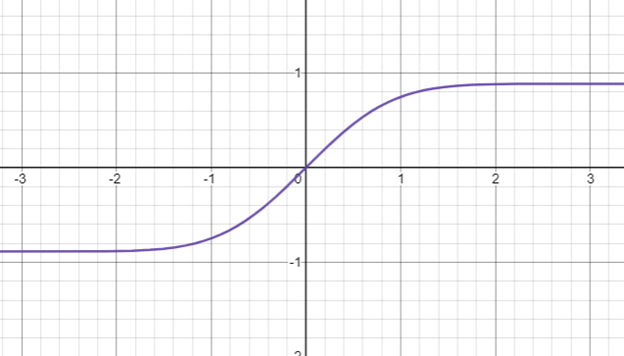
\includegraphics[scale=0.8]{Images/IntegralCalcPictures/AreaOfBellCurve.png}}
This function is the area of the bell curve. The error function $\erf x$, is based on this and is defined as
$$\erf x=\frac{2}{\sqrt{\pi}}\int_0^xe^{-t^2}dt$$
Some other notable functions include:
\begin{align*}
    &\mathrm{C}(x)=\int_0^x\cos(t^2)dt\\
    &\mathrm{S}(x)=\int_0^x\sin(t^2)dt\\
    &\mathrm{H}(x)=\int_0^x\frac{\sin t}{t}dt\\
    &\mathrm{Li}(x)=\int_2^x\frac{dt}{\ln t}\\
    &\Gamma(x)=\int_0^xe^{-t}t^{x-1}dt
\end{align*}
Where $\mathrm{Li}(x)$ is approximately the number of primes less than $x$.\\
and $\Gamma(x)$ is the same as $(x-1)!$